
\subsection{Dataset and Evaluation Method}
The dataset we used in our experiments is provided by StackOverflow.com. Currently, there are 2.2 million questions, 4.8 millions answers, over 35 thousands tags in this dataset\cite{DataDump}.

We prepared 1,050,000 posts(a post is either a question or an answer)  as the training data $S_{train}$, and randomly sampled 500 posts along the timeline as our test dataset $S_{test}$.

We use the precision and recall as the metrics to evaluation the classification methods.
$$ \text{Precision}=\frac{tp}{tp+fp} $$
$$ \text{Recall}=\frac{tp}{tp+fn} $$
where $tp$ is the count of true positive, $fp$ the false positive and $fn$ the false negative.

Currently we manually check the precision of the predicted tags in the test set. This is quite a challenging work because as we discussed in introduction, tags are often quite subjective and incomplete. So it will be inappropriate to require our predicted tags to be exactly the same as the user-defined tags. Thus, we should read the questions and measure the quality of the tag by common sense. 

In this mile-stone, we manually check the results of naive Bayes classifier. In the next step, we will also trying to develop some tools that could ease our checking process. For example, now we have developed a tag similarity calculator based on Kullback-Leibler distance, a method that could determine how similar two 
distributions. In our case, each tag will have a corresponding word distribution $P(word|tag)$. Similar tags often have similar word distribution. For example, the $Distance(eclipse, java)$ is small while $Distance(lisp, eclipse)$ is much bigger.

With these tool we hope in the next step we can semi-automate or automate the evaluation process.

\subsection{Experimental Results}
\subsubsection{Naive Bayes}
In naive Bayes, we choose the top-rank $N$ tags as our predicted tags. Figure \ref{fig:naive} shows the precision/recall of Bayes classifier with different $N$. We can see that the recall increases as $N$ goes up; whereas the precision drops when $N$ increases.

\begin{figure}[htb!]
\centering%
    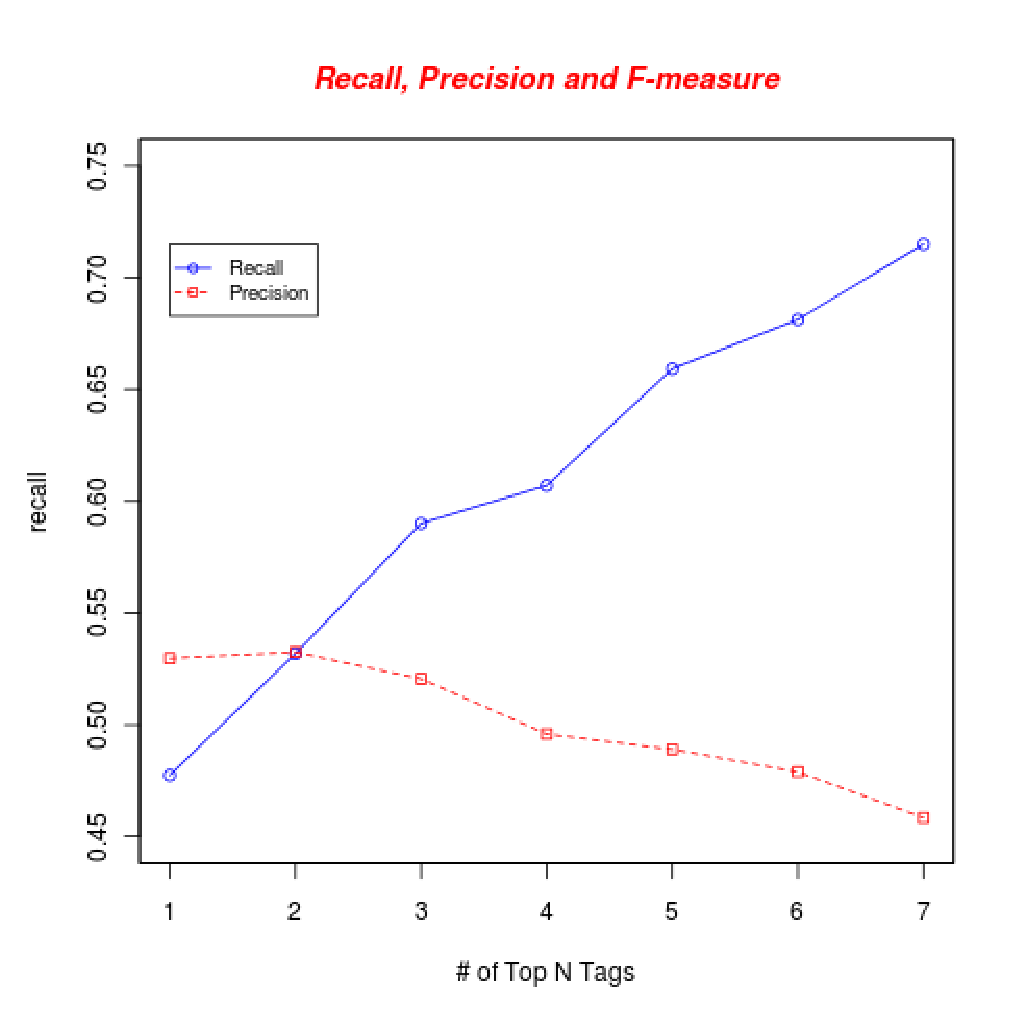
\includegraphics[scale=0.42]{naives.eps}
\caption{Tag Prediction By Naive Bayes}
\label{fig:naive}
\end{figure}

\subsubsection{Logistic Regression}
Under Construction

\subsubsection{Neural Networks}
Under Construction

\subsection{Comparison and Conclusion}
Under Construction. This part depends on the experimental results of all the three models.
